\chapter{Phương pháp nghiên cứu}
\label{chap:methodology}

% ============================================
% CHAPTER 3: METHODOLOGY
% ============================================
% Task 2.11-2.14: Viết Chapter 3 (15-20 pages)
% Trình bày chi tiết experimental protocol, RQs, pipeline, evaluation

\section{Tổng quan phương pháp}
\label{sec:methodology-overview}

Luận văn này thực hiện một \textit{empirical benchmarking study} (nghiên cứu đánh giá thực nghiệm) nhằm so sánh ba phương pháp phát hiện bất thường trên log đại diện cho ba thế hệ machine learning: Classical ML (LightAD), Deep Learning (LogFormer), và LLM (LogRAG). 

\textbf{Loại nghiên cứu:} Quantitative empirical study tuân theo ACM SIGSOFT Empirical Standards \cite{acm_empirical_standards}.

\subsection{Mục tiêu nghiên cứu}
\label{subsec:research-goals}

\textbf{Mục tiêu chính:} Trả lời câu hỏi: "\textit{Phương pháp nào là lựa chọn tốt nhất cho log anomaly detection trong thực tế, xét trên nhiều tiêu chí: hiệu quả, chi phí, và khả năng giải thích?}"

\textbf{Khác biệt so với các nghiên cứu trước:}
\begin{itemize}
    \item \textbf{Cross-generational comparison:} Đầu tiên so sánh hệ thống ba thế hệ ML (Classical, DL, LLM) trên cùng datasets
    \item \textbf{Multi-dimensional evaluation:} Không chỉ accuracy, mà cả computational cost, explainability, error patterns
    \item \textbf{Fair protocol:} Cùng data splits, cùng hardware, cùng metrics
    \item \textbf{Practical guidelines:} Khuyến nghị triển khai dựa trên kết quả thực nghiệm
\end{itemize}

\subsection{Tiếp cận theo RQ (Research Questions)}
\label{subsec:rq-driven}

Nghiên cứu được tổ chức xung quanh 4 Research Questions (RQ), từ hiệu quả đến chi phí, trade-offs, và explainability. Mỗi RQ có metrics và phương pháp đánh giá cụ thể, được trình bày chi tiết trong Section \ref{sec:research-questions}.

\section{Câu hỏi nghiên cứu}
\label{sec:research-questions}

\subsection{RQ1: Hiệu quả phát hiện bất thường}
\label{subsec:rq1}

\textbf{Research Question 1:}

\begin{quote}
\textit{Hiệu quả phát hiện bất thường (detection effectiveness) của LightAD, LogFormer, và LogRAG là bao nhiêu khi đánh giá trên HDFS\_v1 và BGL datasets?}
\end{quote}

\subsubsection{Động lực}

Hiệu quả phát hiện là tiêu chí quan trọng nhất. Một phương pháp không phát hiện được anomaly (low Recall) hoặc tạo ra quá nhiều false alarms (low Precision) đều không khả thi trong production.

\subsubsection{Metrics}

Chúng tôi đo lường hiệu quả qua 5 metrics:

\begin{enumerate}
    \item \textbf{Precision (P):} Tỷ lệ dự đoán anomaly chính xác
    \[
    P = \frac{TP}{TP + FP}
    \]
    \textit{Ý nghĩa:} P cao = ít false alarms = ít "alert fatigue"
    
    \item \textbf{Recall (R):} Tỷ lệ anomaly được phát hiện
    \[
    R = \frac{TP}{TP + FN}
    \]
    \textit{Ý nghĩa:} R cao = ít anomaly bị bỏ sót = ít incidents
    
    \item \textbf{F1-Score (F1):} Harmonic mean của P và R
    \[
    F1 = \frac{2 \cdot P \cdot R}{P + R}
    \]
    \textit{Ý nghĩa:} F1 cân bằng Precision và Recall, metric chính để ranking methods
    
    \item \textbf{PR-AUC:} Area under Precision-Recall curve
    
    \textit{Ý nghĩa:} Đánh giá performance across all thresholds, robust với imbalanced data
    
    \item \textbf{FPR:} False Positive Rate
    \[
    FPR = \frac{FP}{FP + TN}
    \]
    \textit{Ý nghĩa:} FPR < 1\% thường được chấp nhận trong industry (target)
\end{enumerate}

\subsubsection{Kỳ vọng}

\textbf{Hypothesis:} Deep Learning và LLM methods (LogFormer, LogRAG) sẽ có F1 và PR-AUC cao hơn Classical ML (LightAD), nhưng sự khác biệt có thể không lớn trên datasets đơn giản như HDFS\_v1.

\textbf{Insight mong đợi:} Xác định phương pháp nào có accuracy cao nhất, và liệu classical ML có "competitive" hay không (theo tuyên bố của LightAD paper \cite{yu2024lightad}).

\subsection{RQ2: Chi phí tính toán}
\label{subsec:rq2}

\textbf{Research Question 2:}

\begin{quote}
\textit{Chi phí tính toán (computational cost) của mỗi phương pháp là bao nhiêu, bao gồm training time, inference latency, memory usage, và throughput?}
\end{quote}

\subsubsection{Động lực}

Accuracy không phải là tiêu chí duy nhất. Một phương pháp với F1 = 0.98 nhưng inference time 10 seconds/sample không thể triển khai trong real-time system. Chi phí cũng bao gồm API cost cho LLM-based methods.

\subsubsection{Metrics}

\begin{enumerate}
    \item \textbf{Training Time:} Thời gian huấn luyện model từ đầu (wall-clock time)
    
    \textit{Measured:} Seconds (s) hoặc Hours (h)
    
    \textit{Ý nghĩa:} Quan trọng khi cần retrain thường xuyên (concept drift)
    
    \item \textbf{Inference Latency:} Thời gian dự đoán một sample
    
    \textit{Measured:} Milliseconds (ms), report mean, p95, p99
    
    \textit{Ý nghĩa:} Critical cho real-time systems (target: < 100ms/sample)
    
    \item \textbf{Memory Usage:}
    \begin{itemize}
        \item \textbf{Peak RAM:} System memory (GB)
        \item \textbf{Peak VRAM:} GPU memory (GB)
    \end{itemize}
    
    \textit{Ý nghĩa:} Quan trọng cho resource-constrained environments
    
    \item \textbf{Throughput:} Số samples xử lý mỗi giây
    
    \textit{Measured:} Samples/second
    
    \textit{Ý nghĩa:} Quan trọng cho high-velocity log streams (millions logs/hour)
    
    \item \textbf{API Cost (LogRAG only):} Chi phí OpenAI API
    
    \textit{Measured:} USD per 1K samples
    
    \textit{Ý nghĩa:} Operational cost cho LLM-based methods
\end{enumerate}

\subsubsection{Phương pháp đo}

\begin{itemize}
    \item \textbf{Hardware cố định:} NVIDIA RTX 3090 (24GB VRAM), Intel Core i9, 32GB RAM
    \item \textbf{Monitoring tools:} 
        \begin{itemize}
            \item \texttt{nvidia-smi} cho GPU metrics
            \item \texttt{psutil} (Python) cho RAM
            \item \texttt{time.perf\_counter()} cho wall-clock time
        \end{itemize}
    \item \textbf{Repeated runs:} Mỗi measurement chạy 5 lần, report mean $\pm$ std
\end{itemize}

\subsubsection{Kỳ vọng}

\textbf{Hypothesis:} 
\begin{itemize}
    \item Training time: LightAD < LogFormer < LogRAG (không có pre-training overhead)
    \item Inference latency: LightAD (DT) < LogFormer < LogRAG (API calls)
    \item Memory: LightAD < LogFormer < LogRAG
    \item API cost: LogRAG đắt nhất (GPT-3.5: \$0.002/1K tokens)
\end{itemize}

\textbf{Insight mong đợi:} Quantify chi phí của deep learning và LLM so với classical ML. Xác định liệu classical ML có "efficiency advantage" đáng kể hay không.

\subsection{RQ3: Đánh đổi hiệu năng-chi phí}
\label{subsec:rq3}

\textbf{Research Question 3:}

\begin{quote}
\textit{Đánh đổi (trade-offs) giữa detection effectiveness (RQ1) và computational cost (RQ2) là gì? Phương pháp nào nằm trên Pareto frontier?}
\end{quote}

\subsubsection{Động lực}

Trong thực tế, lựa chọn phương pháp phụ thuộc vào deployment constraints:
\begin{itemize}
    \item High-stakes production (banking, healthcare): Ưu tiên accuracy
    \item Real-time systems (network monitoring): Ưu tiên latency
    \item Resource-constrained (edge devices): Ưu tiên memory
\end{itemize}

RQ3 cung cấp trade-off analysis để hỗ trợ decision-making.

\subsubsection{Phương pháp phân tích}

\textbf{Pareto Frontier Analysis:}

\begin{enumerate}
    \item Vẽ scatter plots: 
    \begin{itemize}
        \item X-axis: Inference latency (ms)
        \item Y-axis: F1-Score
    \end{itemize}
    
    \item Xác định Pareto-optimal points: Phương pháp $A$ dominates $B$ nếu:
    \[
    F1_A \geq F1_B \quad \text{AND} \quad \text{Latency}_A \leq \text{Latency}_B
    \]
    với ít nhất một inequality strict.
    
    \item Phương pháp trên Pareto frontier là optimal trade-off (không thể improve một metric mà không sacrifice metric kia)
\end{enumerate}

\textbf{Multi-dimensional comparison:}
\begin{itemize}
    \item Radar charts: So sánh 3 methods trên 5 dimensions (F1, Speed, Memory, Cost, Explainability)
    \item Normalize mỗi dimension về 0-1 scale
\end{itemize}

\subsubsection{Kỳ vọng}

\textbf{Hypothesis:}
\begin{itemize}
    \item LightAD-DT có thể là Pareto-optimal: Good F1 + Very low latency
    \item LogFormer: Higher F1 nhưng moderate latency
    \item LogRAG: Highest F1 nhưng highest latency và cost
\end{itemize}

\textbf{Insight mong đợi:} Decision tree để chọn phương pháp dựa trên use case constraints.

\subsection{RQ4: Khả năng giải thích và phân tích lỗi}
\label{subsec:rq4}

\textbf{Research Question 4:}

\begin{quote}
\textit{Các error patterns (FP/FN) của mỗi phương pháp là gì? Khả năng giải thích (explainability) của predictions như thế nào?}
\end{quote}

\subsubsection{Động lực}

\textbf{Phần (a) - Error Analysis:} Hiểu \textit{tại sao} một phương pháp fail giúp:
\begin{itemize}
    \item Identify weaknesses (e.g., poor on rare templates)
    \item Guide method selection (e.g., avoid method X nếu dataset có characteristic Y)
    \item Future improvements (e.g., hybrid approaches)
\end{itemize}

\textbf{Phần (b) - Explainability:} Trong production, SREs cần biết \textit{tại sao} một log được classify as anomaly. Black-box predictions không được trust.

\subsubsection{Phương pháp}

\textbf{(a) Error Analysis:}

\begin{enumerate}
    \item \textbf{Extract errors:} Từ test set, lấy 50-100 False Positives (FP) và 50-100 False Negatives (FN) của mỗi phương pháp.
    
    \item \textbf{Build error taxonomy:} Classify errors vào các categories:
    \begin{itemize}
        \item \textit{Unseen template:} Log template chưa thấy trong training (rare event)
        \item \textit{Short sequence:} Sequence quá ngắn, thiếu context
        \item \textit{Noise:} Parsing errors, malformed logs
        \item \textit{Class imbalance:} Minority class bị underrepresented
        \item \textit{Semantic ambiguity:} Log trông bình thường nhưng thực tế bất thường (hoặc ngược lại)
    \end{itemize}
    
    \item \textbf{Quantify distribution:} Tính phần trăm mỗi error category cho mỗi phương pháp.
    
    \item \textbf{Case studies:} Phân tích chi tiết 2-3 FP và 2-3 FN examples mỗi phương pháp.
\end{enumerate}

\textbf{(b) Explainability Analysis:}

\begin{enumerate}
    \item \textbf{Extract explanations:}
    \begin{itemize}
        \item \textbf{LightAD-KNN:} Show k nearest neighbors
        \item \textbf{LightAD-DT:} Show decision path (which rules applied)
        \item \textbf{LightAD-SLFN:} Feature importance (top features)
        \item \textbf{LogFormer:} Attention weights (which log events attended)
        \item \textbf{LogRAG:} Retrieved examples + LLM reasoning chain
    \end{itemize}
    
    \item \textbf{Assess explainability criteria:}
    \begin{itemize}
        \item \textit{Actionability:} Liệu SRE có thể sử dụng explanation để debug? (1-5 scale)
        \item \textit{Clarity:} Explanation có dễ hiểu với non-ML expert? (1-5 scale)
        \item \textit{Correctness:} Explanation có align với root cause thực tế? (1-5 scale)
    \end{itemize}
    
    \item \textbf{Visualizations:}
    \begin{itemize}
        \item Decision tree diagram (LightAD-DT)
        \item Attention heatmap (LogFormer)
        \item Retrieved examples + reasoning chain (LogRAG)
    \end{itemize}
\end{enumerate}

\subsubsection{Kỳ vọng}

\textbf{Hypothesis:}
\begin{itemize}
    \item \textbf{Error patterns:} 
        \begin{itemize}
            \item LightAD: Nhiều errors trên rare templates (limited training data)
            \item LogFormer: Ít errors hơn do pre-training (learned general patterns)
            \item LogRAG: Ít FN (high Recall) nhưng có thể nhiều FP (over-sensitive)
        \end{itemize}
    \item \textbf{Explainability:}
        \begin{itemize}
            \item LightAD-DT: Best (clear if-then rules)
            \item LogRAG: Best for non-ML users (natural language)
            \item LogFormer: Moderate (attention weights need expertise)
        \end{itemize}
\end{itemize}

\textbf{Insight mong đợi:} 
\begin{itemize}
    \item Identify which method is best for explainability-critical applications
    \item Common failure modes across methods (guide future work)
\end{itemize}

\section{Pipeline thực nghiệm}
\label{sec:experimental-pipeline}

\subsection{Quy trình end-to-end}
\label{subsec:pipeline-overview}

Hình \ref{fig:pipeline} minh họa pipeline thực nghiệm 5 bước:

\begin{figure}[ht]
\centering
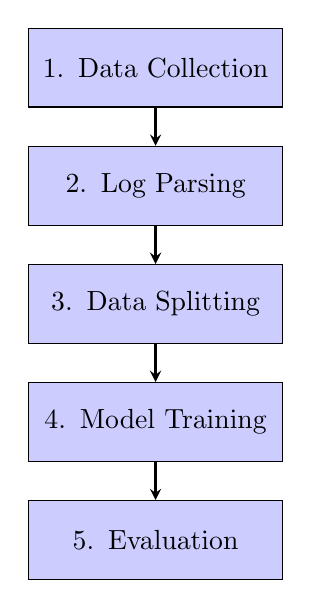
\begin{tikzpicture}[
    node distance=1.5cm,
    box/.style={rectangle, draw, fill=blue!20, text width=3cm, text centered, minimum height=1cm},
    arrow/.style={->, >=stealth, thick}
]
    \node[box] (collect) {1. Data Collection};
    \node[box, below of=collect] (parse) {2. Log Parsing};
    \node[box, below of=parse] (split) {3. Data Splitting};
    \node[box, below of=split] (train) {4. Model Training};
    \node[box, below of=train] (eval) {5. Evaluation};
    
    \draw[arrow] (collect) -- (parse);
    \draw[arrow] (parse) -- (split);
    \draw[arrow] (split) -- (train);
    \draw[arrow] (train) -- (eval);
\end{tikzpicture}
\caption{Pipeline thực nghiệm 5 bước}
\label{fig:pipeline}
\end{figure}

\subsubsection{Step 1: Data Collection}

\textbf{Datasets:} HDFS\_v1 và BGL từ LogHub \cite{he2020loghub}.

\textbf{Characteristics:} Đã trình bày chi tiết trong Section \ref{subsec:datasets} (Chapter 2).

\textbf{Download:}
\begin{itemize}
    \item \textbf{HDFS\_v1:} \url{https://zenodo.org/record/8196385}
    \item \textbf{BGL:} \url{https://zenodo.org/record/8196385}
\end{itemize}

\textbf{Verification:} Checksum verification để đảm bảo data integrity.

\subsubsection{Step 2: Log Parsing}

\textbf{Tool:} Drain3 \cite{he2017drain} - state-of-art log parser.

\textbf{Purpose:} Chuyển đổi raw logs thành structured format:
\begin{itemize}
    \item \textbf{Input:} Raw log line (semi-structured text)
    \item \textbf{Output:} 
        \begin{itemize}
            \item \textit{Template ID:} Integer representing log event type
            \item \textit{Template:} Template string (với <*> cho parameters)
            \item \textit{Parameters:} Extracted variable values
        \end{itemize}
\end{itemize}

\textbf{Example:}
\begin{verbatim}
Input:  "2024-01-15 10:23:45 ERROR Connection to 192.168.1.1 failed"
Output: {
    "template_id": 42,
    "template": "ERROR Connection to <*> failed",
    "parameters": ["192.168.1.1"],
    "timestamp": "2024-01-15 10:23:45"
}
\end{verbatim}

\textbf{Configuration:}
\begin{itemize}
    \item \textbf{Depth:} 4 (Drain tree depth)
    \item \textbf{Similarity threshold:} 0.5
    \item \textbf{Max children:} 100
\end{itemize}

\textbf{Output:}
\begin{itemize}
    \item \texttt{hdfs\_structured.jsonl} (575K blocks)
    \item \texttt{bgl\_structured.jsonl} (4.3M log lines)
    \item Template dictionaries với frequencies
\end{itemize}

\subsubsection{Step 3: Data Splitting}

\textbf{Ratio:} 80\% training, 10\% validation, 10\% test

\textbf{Strategy:} Khác nhau cho mỗi dataset để tránh data leakage và ensure temporal validity.

\paragraph{HDFS\_v1: Block-based Splitting}

\begin{itemize}
    \item \textbf{Grouping:} Mỗi block ID là một session
    \item \textbf{Label:} Block anomalous nếu bất kỳ log nào trong block là anomalous
    \item \textbf{Splitting:} Stratified split theo label (giữ anomaly ratio)
    \item \textbf{Rationale:} Tránh leakage - logs từ cùng block không được tách ra train/test
\end{itemize}

\textbf{Algorithm:}
\begin{verbatim}
1. Group logs by BlockId
2. Aggregate label: Block anomalous if max(log labels) = 1
3. Stratified split by block label:
   - Train: 80% blocks (stratified)
   - Val: 10% blocks (stratified)
   - Test: 10% blocks (stratified)
\end{verbatim}

\paragraph{BGL: Chronological Splitting}

\begin{itemize}
    \item \textbf{Grouping:} Sliding window (20 consecutive logs)
    \item \textbf{Label:} Window anomalous nếu bất kỳ log nào bất thường
    \item \textbf{Splitting:} Chronological (first 80\% → train, next 10\% → val, last 10\% → test)
    \item \textbf{Rationale:} Preserve temporal order, test on future data (realistic deployment)
\end{itemize}

\textbf{Algorithm:}
\begin{verbatim}
1. Sort logs by timestamp
2. Create sliding windows (size=20, step=10)
3. Label window: Anomalous if any(log labels) = 1
4. Chronological split:
   - Train: Windows 0 to 80%
   - Val: Windows 80% to 90%
   - Test: Windows 90% to 100%
\end{verbatim}

\textbf{Verification:}
\begin{itemize}
    \item Check no overlap between train/val/test
    \item Verify anomaly rates similar across splits (±2\%)
    \item Document split statistics
\end{itemize}

\subsubsection{Step 4: Model Training}

\textbf{Seed:} Fixed random seed = 42 cho reproducibility

\textbf{Hyperparameters:}
\begin{itemize}
    \item \textbf{Start:} Paper defaults cho mỗi phương pháp
    \item \textbf{Tuning:} Chỉ tune trên validation set
    \item \textbf{Rule:} \textbf{NEVER} touch test set (no peeking!)
\end{itemize}

\paragraph{LightAD Training}

\begin{itemize}
    \item \textbf{Feature representation:} Event count vector
    \item \textbf{Models:}
        \begin{itemize}
            \item KNN: k=5 (default from paper)
            \item Decision Tree: max\_depth=10, min\_samples\_split=20
            \item SLFN: hidden\_units=50, epochs=100, lr=0.001
        \end{itemize}
    \item \textbf{Training time:} Minutes (< 10 min expected)
\end{itemize}

\paragraph{LogFormer Training}

\begin{itemize}
    \item \textbf{Phase 1: Pre-training (optional - use pretrained BigLog model)}
        \begin{itemize}
            \item Model: BERT-base architecture
            \item Corpus: BigLog (100M logs)
            \item Task: Masked Language Modeling
        \end{itemize}
    \item \textbf{Phase 2: Adapter Tuning}
        \begin{itemize}
            \item Adapter config: bottleneck dim = 64
            \item Epochs: 10 (tune on val set)
            \item Batch size: 32
            \item Learning rate: 1e-4
        \end{itemize}
    \item \textbf{Training time:} Hours (4-8 hours on RTX 3090)
\end{itemize}

\paragraph{LogRAG Training}

\begin{itemize}
    \item \textbf{Phase 1: DeepSVDD}
        \begin{itemize}
            \item Encoder: 3-layer MLP [128, 64, 32]
            \item Hypersphere center: Initialized from mean of normal samples
            \item Epochs: 50
            \item Learning rate: 0.0001
        \end{itemize}
    \item \textbf{Phase 2: RAG Setup}
        \begin{itemize}
            \item Retriever: FAISS index (Flat L2)
            \item Top-k: 5 retrieved examples
            \item LLM: GPT-3.5-turbo (OpenAI API) hoặc Mistral-7B (local)
        \end{itemize}
    \item \textbf{Training time:} Hours (DeepSVDD: 2-4 hours, no LLM training)
\end{itemize}

\subsubsection{Step 5: Evaluation}

\textbf{Test set:} Chỉ sử dụng sau khi model đã fixed (no tuning on test!)

\textbf{Metrics:} Compute all metrics từ RQ1 (Precision, Recall, F1, PR-AUC, FPR)

\textbf{Statistical testing:} Wilcoxon signed-rank test cho pairwise comparisons (significant if p < 0.05)

\textbf{Repeated runs:} 5 runs với different seeds (42, 123, 456, 789, 2024), report mean ± std

\subsection{Kiểm soát công bằng}
\label{subsec:fairness-controls}

Để đảm bảo so sánh công bằng giữa 3 phương pháp, chúng tôi kiểm soát các factors sau:

\subsubsection{Phần cứng thống nhất}

\textbf{Hardware configuration:}
\begin{itemize}
    \item \textbf{GPU:} NVIDIA RTX 3090 (24GB VRAM)
    \item \textbf{CPU:} Intel Core i9-12900K
    \item \textbf{RAM:} 32GB DDR4
    \item \textbf{Storage:} 1TB NVMe SSD
    \item \textbf{OS:} Ubuntu 22.04 LTS
\end{itemize}

\textbf{Rationale:} Eliminate hardware confounding factor. Tất cả methods chạy trên cùng machine.

\subsubsection{Seed cố định}

\textbf{Random seed = 42} cho:
\begin{itemize}
    \item Data splitting (train/val/test)
    \item Model initialization
    \item Stochastic training procedures
\end{itemize}

\textbf{Rationale:} Reproducibility và eliminate randomness.

\textbf{Multiple runs:} Chạy 5 lần với 5 seeds khác nhau (42, 123, 456, 789, 2024) để estimate variance.

\subsubsection{Hyperparameters}

\textbf{Protocol:}
\begin{enumerate}
    \item \textbf{Start:} Paper defaults cho mỗi method
    \item \textbf{Tuning:} Nếu cần tune, chỉ tune trên validation set
    \item \textbf{Rule:} No peeking at test set
    \item \textbf{Document:} Ghi lại tất cả hyperparameters trong appendix
\end{enumerate}

\textbf{Rationale:} Fair comparison - no cherry-picking hyperparameters to favor one method.

\subsubsection{Evaluation protocol}

\textbf{Same for all methods:}
\begin{itemize}
    \item Same data splits (train/val/test)
    \item Same metrics (P/R/F1/PR-AUC/FPR)
    \item Same evaluation script (unified \texttt{evaluate.py})
    \item Same statistical tests
\end{itemize}

\textbf{Rationale:} Apples-to-apples comparison.

\section{Giao thức tái lập}
\label{sec:reproducibility}

Chúng tôi cam kết reproducibility theo ACM Artifact Review and Badging guidelines \cite{acm_artifact_badging}.

\subsection{Code release}

\textbf{GitHub repository:} Public repository chứa:
\begin{itemize}
    \item All scripts (parsing, training, evaluation, visualization)
    \item Configuration files (hyperparameters)
    \item Data processing code
    \item Jupyter notebooks cho analysis
\end{itemize}

\textbf{License:} MIT License (permissive open-source)

\subsection{Data availability}

\textbf{Datasets:} Links đến LogHub (HDFS\_v1, BGL)

\textbf{Processed data:} Parsed logs và splits sẽ được host trên Zenodo (DOI)

\textbf{Privacy:} Cả hai datasets đều public, không có privacy concerns.

\subsection{Environment}

\textbf{Docker container:} Dockerfile để recreate exact environment:
\begin{itemize}
    \item Python 3.8
    \item PyTorch 1.13.1
    \item Transformers 4.30.0
    \item All dependencies với pinned versions
\end{itemize}

\textbf{Quick start:}
\begin{verbatim}
docker pull <username>/logad-bench:v1.0
docker run --gpus all -v $(pwd):/workspace <image>
bash scripts/run_all_experiments.sh
\end{verbatim}

\subsection{Results package}

\textbf{Contents:}
\begin{itemize}
    \item Raw results (JSON files với tất cả metrics)
    \item Trained model checkpoints (nếu khả thi, exclude LogRAG do API)
    \item Analysis scripts (reproduce figures và tables)
    \item LaTeX source cho thesis chapters
\end{itemize}

\textbf{Goal:} Any researcher có thể reproduce mọi figure và table trong thesis.

\section{Threats to Validity}
\label{sec:threats-to-validity}

Theo ACM Empirical Standards, chúng tôi identify và mitigate các threats to validity:

\subsection{Internal Validity}

\textbf{Threat 1: Implementation bugs}

\textit{Mitigation:}
\begin{itemize}
    \item Sử dụng official implementations (LightAD, LogFormer, LogRAG GitHub repos)
    \item Unit tests cho data processing code
    \item Sanity checks (e.g., metrics in reasonable range)
\end{itemize}

\textbf{Threat 2: Hyperparameter tuning bias}

\textit{Mitigation:}
\begin{itemize}
    \item Start from paper defaults
    \item Document all tuning decisions
    \item Tune only on validation set, never test set
\end{itemize}

\textbf{Threat 3: Random variation}

\textit{Mitigation:}
\begin{itemize}
    \item Fixed random seeds
    \item Multiple runs (5 seeds)
    \item Report mean ± std
    \item Statistical significance testing
\end{itemize}

\subsection{External Validity}

\textbf{Threat 1: Limited datasets}

\textit{Discussion:} Chỉ 2 datasets (HDFS\_v1, BGL). Results có thể không generalize sang hệ thống khác.

\textit{Mitigation:}
\begin{itemize}
    \item Chọn 2 datasets representative: HDFS (simple, structured) vs BGL (complex, diverse)
    \item Acknowledge limitation trong discussion
    \item Future work: Extend to more datasets
\end{itemize}

\textbf{Threat 2: Specific versions}

\textit{Discussion:} Kết quả dựa trên specific versions của LightAD, LogFormer, LogRAG. Newer versions có thể khác.

\textit{Mitigation:}
\begin{itemize}
    \item Document exact versions và commit hashes
    \item Pin dependencies trong Docker
    \item Acknowledge limitation
\end{itemize}

\subsection{Construct Validity}

\textbf{Threat 1: Metric choices}

\textit{Discussion:} Liệu F1, PR-AUC có phải best metrics cho LogAD?

\textit{Mitigation:}
\begin{itemize}
    \item F1 và PR-AUC widely accepted trong LogAD literature
    \item Report multiple metrics (5 total) để triangulate
    \item RQ4 provides qualitative analysis (error patterns)
\end{itemize}

\textbf{Threat 2: Explainability assessment}

\textit{Discussion:} Actionability, Clarity, Correctness là subjective (assessed by authors).

\textit{Mitigation:}
\begin{itemize}
    \item Provide concrete examples (case studies)
    \item Document assessment criteria clearly
    \item Acknowledge subjectivity
    \item Future work: User study với SREs
\end{itemize}

\section{Kết luận}
\label{sec:methodology-conclusion}

Chương này đã trình bày:
\begin{enumerate}
    \item \textbf{4 Research Questions:} RQ1 (Effectiveness), RQ2 (Cost), RQ3 (Trade-offs), RQ4 (Explainability + Errors)
    \item \textbf{Experimental pipeline:} 5 bước từ data collection đến evaluation
    \item \textbf{Fairness controls:} Same hardware, seeds, hyperparameter protocol, evaluation metrics
    \item \textbf{Reproducibility protocol:} Code, data, environment, results package
    \item \textbf{Threats to validity:} Identified và mitigated
\end{enumerate}

Chương tiếp theo (Chapter 4) sẽ trình bày kết quả thực nghiệm, trả lời từng Research Question với data và visualizations.
